\documentclass{beamer}

\usepackage[T1]{fontenc}
\usepackage[utf8]{inputenc}
\usepackage[polish]{babel}
\usepackage{lmodern}
\usepackage{booktabs}

\usepackage{tikz}
\usetikzlibrary{positioning, arrows.meta, fit}


\usetheme{Madrid}
\usecolortheme{default}

%------------------------------------------------------------
%This block of code defines the information to appear in the
%Title page
\title[Odczyt tablicy rejestracyjnej]{Odczytywanie tablicy rejestracyjnej ze zdjęcia}

\subtitle{Deep learning w Chmurze}

\author{Joanna Dagil \and Maja Szerszeń}

\date{\today}

%\logo{\includegraphics[height=1cm]{overleaf-logo}}

%End of title page configuration block
%------------------------------------------------------------



%------------------------------------------------------------
%The next block of commands puts the table of contents at the
%beginning of each section and highlights the current section:

% \AtBeginSection[]
% {
%   \begin{frame}
%     \frametitle{Spis treści}
%     \tableofcontents[currentsection]
%   \end{frame}
% }
%------------------------------------------------------------


\begin{document}

%The next statement creates the title page.
\frame{\titlepage}


%---------------------------------------------------------
%This block of code is for the table of contents after
%the title page
\begin{frame}
\frametitle{Spis treści}
\tableofcontents
\end{frame}
%---------------------------------------------------------


\section{Streszczenie}

\begin{frame}{Streszczenie}


    Celem projektu jest automatyczne \textbf{odczytanie numeru tablicy rejestracyjnej} z fotografii pojazdu.

    \vspace{0.3cm}

    Zastosowano \textbf{podejście dwustopniowe}: najpierw detekcja tablicy na zdjęciu, następnie rozpoznanie pojedynczych znaków.

    Oba etapy oparto na modelu \texttt{YOLO11} (Ultralytics); całość trenowana i uruchamiana w \textbf{środowisku chmurowym} (Kaggle / Colab, GPU Tesla~T4).
    
    \vspace{0.3cm}

    Kluczowy pomysł: detektor znaków wzmocniono \textbf{danymi syntetycznymi} (generator tablic z automatycznymi bounding boxami) oraz \textbf{pseudo-etykietowaniem} prawdziwych cropów.

    \vspace{0.3cm}

    Wyniki: detekcja tablicy \textbf{mAP@0.5 = 0{,}97}, odczyt całej tablicy \textbf{exact match $\approx$ 61\%}, błąd na poziomie znaku \textbf{CER $\approx$ 0{,}15}.

\end{frame}



%---------------------------------------------------------


%---------------------------------------------------------

\section{Wstęp / wprowadzenie}

\begin{frame}{Wstęp / wprowadzenie}

\textbf{Automatyczne rozpoznawanie tablic rejestracyjnych} (ANPR) jest powszechnie
stosowane w systemach parkingowych, kontroli dostępu, pobierania opłat drogowych
i monitoringu ruchu.

\vspace{0.3cm}

Zadanie jest trudne, ponieważ na zdjęciach występują:
\begin{itemize}
    \item różne kąty, perspektywa i krzywizna tablicy,
    \item zmienne warunki oświetleniowe oraz niska rozdzielczość,
    \item rozmycie, szum i artefakty kompresji,
    \item podobne do siebie znaki (np. \texttt{O}/\texttt{0}, \texttt{Q}/\texttt{O},
    \texttt{X}, \texttt{8}/\texttt{B}).
\end{itemize}

\vspace{0.3cm}

W projekcie sprawdzamy, czy lekkie modele detekcji jednofazowej w połączeniu z danymi syntetycznymi pozwalają zbudować pipeline odczytu tablic.

\end{frame}

%---------------------------------------------------------


%---------------------------------------------------------
\section{Opis kontekstu i celu projektu}


\begin{frame}{Opis kontekstu i celu projektu}

Zbudowanie systemu, który z fotografii pojazdu zwraca ciąg znaków odpowiadający tablicy rejestracyjnej.

\vspace{0.3cm}

\textbf{Cele szczegółowe:}
\begin{itemize}
    \item wytrenowanie detektora położenia tablicy (YOLO11n),
    \item wytrenowanie detektora 36 klas znaków (cyfry 0--9, litery A--Z),
    \item rozwiązanie problemu \textbf{małej liczby oznaczonych znaków} poprzez
    dane syntetyczne i pseudo-etykietowanie,
    \item ilościowa ocena detekcji oraz tekstowa ocena odczytu (exact match, CER).
\end{itemize}

\end{frame}



%---------------------------------------------------------
\section{Literatura}
%---------------------------------------------------------

\begin{frame}{Literatura}

\small

\begin{itemize}
    \item Khanam, R., Hussain, M. (2024).
    \textit{YOLOv11: An Overview of the Key Architectural Enhancements}.
    arXiv:2410.17725.\\
    \url{https://arxiv.org/abs/2410.17725}

    \item Jocher, G., Qiu, J. (2024).
    \textit{Ultralytics YOLO11} (Version 11.0.0) [Computer software].
    GitHub.\\
    \url{https://github.com/ultralytics/ultralytics}

    \item Arbab, B. A. \textit{License Plate Detection Dataset (10,125 Images)}. Kaggle.\\
    \url{https://www.kaggle.com/datasets/barkataliarbab/license-plate-detection-dataset-10125-images}

    \item Yazdani, N. \textit{License Plate Text Recognition Dataset}. Kaggle.\\
    \url{https://www.kaggle.com/datasets/nickyazdani/license-plate-text-recognition-dataset}
\end{itemize}

\end{frame}


%---------------------------------------------------------
\section{Opis danych}
%---------------------------------------------------------


\begin{frame}{Opis danych}

\textbf{Pierwszy zbiór danych} -- \textit{License Plate Detection Dataset (10,125 Images)} zawiera adnotacje lokalizacji tablic na zdjęciu, które pozwalają na \textbf{detekcję} tablicy na obrazie. Nie zawiera jednak oznaczenia faktycznych numerów tablic.

\vspace{0.2cm}

\textbf{Drugi zbiór danych} -- \textit{License Plate Characters - Detection OCR} -- zawiera ok. 200 prawdziwych cropów tablic z etykietami lokalizacyjnymi dla wszystkich zanków. Wykorzystany jako podstawa do klasyfikowania.

\vspace{0.2cm}

Dodatkowo wygenerowałyśmy \textbf{syntetyczny zbiór cropów tablic} poddanych przekształceniom geometrycznym i zniekształceniom.

\vspace{0.2cm}

\textbf{Trzeci zbiór danych} -- \textit{License Plate Text Recognition Dataset} -- zawiera tysiące prawdziwych cropów tablic z etykietami \textbf{tekstowymi} (bez bounding boxów znaków). Wykorzystany do pseudo-etykietowania.

\vspace{0.2cm}

W celu zmierzenia \textbf{jakości odczytywania numerów} posłużyłyśmy się
analizą na \textbf{próbce ręcznie oznaczonych tablic} (\emph{manual ground truth}).

\vspace{0.2cm}

\scriptsize
Dokładniejsze opisy danych przy opisie metody z nich korzystającej.

\end{frame}



%---------------------------------------------------------
\section{Opis metod}
%---------------------------------------------------------

\begin{frame}{Opis metod}

\begin{columns}[T,onlytextwidth]

% LEWA KOLUMNA
\column{0.52\textwidth}

\small
W projekcie zastosowano podejście dwustopniowe, ponieważ problem odczytywania tablicy rejestracyjnej składa się z dwóch zadań:

\begin{itemize}
    \item \textbf{detekcji tablicy} -- znalezienia miejsca, w którym tablica znajduje się na obrazie,
    \item \textbf{rozpoznania tekstu} -- odczytania znaków z wyciętego fragmentu tablicy.
\end{itemize}

% PRAWA KOLUMNA
\column{0.46\textwidth}

\centering

\resizebox{0.9\textwidth}{!}{
\begin{tikzpicture}[
    node distance=0.35cm,
    box/.style={
        rectangle,
        rounded corners,
        draw=blue!60,
        fill=blue!8,
        thick,
        minimum width=3.8cm,
        minimum height=0.65cm,
        align=center,
        font=\scriptsize
    },
    arrow/.style={
        -Latex,
        thick,
        draw=blue!70
    },
    stagebox/.style={
        rectangle,
        rounded corners,
        draw=gray!70,
        dashed,
        thick,
        inner sep=0.18cm
    },
    stagelabel/.style={
        font=\scriptsize\bfseries,
        rotate=90,
        text=gray!80
    }
]

\node[box] (image) {Obraz pojazdu};
\node[box, below=of image] (plateyolo) {YOLO -- detekcja tablicy};
\node[box, below=of plateyolo] (crop) {Crop tablicy};
\node[box, below=of crop] (charyolo) {YOLO -- klasyfikacja znaków};
\node[box, below=of charyolo] (filter) {Filtrowanie detekcji};
\node[box, below=of filter] (sort) {Sortowanie znaków};
\node[box, below=of sort] (text) {Odczytany tekst};

\draw[arrow] (image) -- (plateyolo);
\draw[arrow] (plateyolo) -- (crop);
\draw[arrow] (crop) -- (charyolo);
\draw[arrow] (charyolo) -- (filter);
\draw[arrow] (filter) -- (sort);
\draw[arrow] (sort) -- (text);

% Przerywane ramki etapów
\node[stagebox, fit=(image)(plateyolo)(crop)] (stage1) {};
\node[stagebox, fit=(charyolo)(filter)(sort)(text)] (stage2) {};

% Pionowe etykiety etapów
\node[stagelabel, right=0.15cm of stage1] {Etap 1};
\node[stagelabel, right=0.15cm of stage2] {Etap 2};

\end{tikzpicture}
}

\end{columns}

\end{frame}



%---------------------------------------------------------
\begin{frame}{Etap 1 -- detekcja tablicy (YOLO11n)}

Do wykrywania położenia tablicy rejestracyjnej wykorzystano model \texttt{YOLO11n} z biblioteki Ultralytics.

\begin{itemize}
    \item YOLO jest jednofazowym (one-stage) modelem detekcji obiektów.
    \item Model uczony był detekcji jednej klasy: \texttt{License\_Plate}.
    \item Zwraca ramki ograniczające (\textit{bounding box}) oraz poziom pewności
    detekcji (\textit{confidence score}).
    \item Wybrano wariant \texttt{YOLO11n} (nano, $\sim$2{,}6~mln parametrów),
    ponieważ jest lekki i szybki, co ułatwia eksperymenty w chmurze.
\end{itemize}

\vspace{0.2cm}

\footnotesize
\textbf{Konfiguracja treningu:} 30 epok, \texttt{imgsz} = 640, \texttt{batch} = 16,
wagi startowe \texttt{yolo11n.pt}, \texttt{patience} = 10.

\end{frame}

%---------------------------------------------------------

\begin{frame}{\textit{License Plate Detection Dataset (10,125 Images)}}

\begin{columns}

\column{0.60\textwidth}

Zdjęcia pojazdów z oznaczonym położeniem tablic rejestracyjnych.

\vspace{0.2cm}

Dane są zapisane w formacie zgodnym z YOLO.
Dla każdego obrazu istnieje odpowiadający mu plik tekstowy z etykietą.

\vspace{0.2cm}

\footnotesize
Podział: \textbf{train} / \textbf{valid} (2048 obrazów) / \textbf{test} (1020 obrazów),
jedna klasa: \texttt{License\_Plate}.

\column{0.40\textwidth}

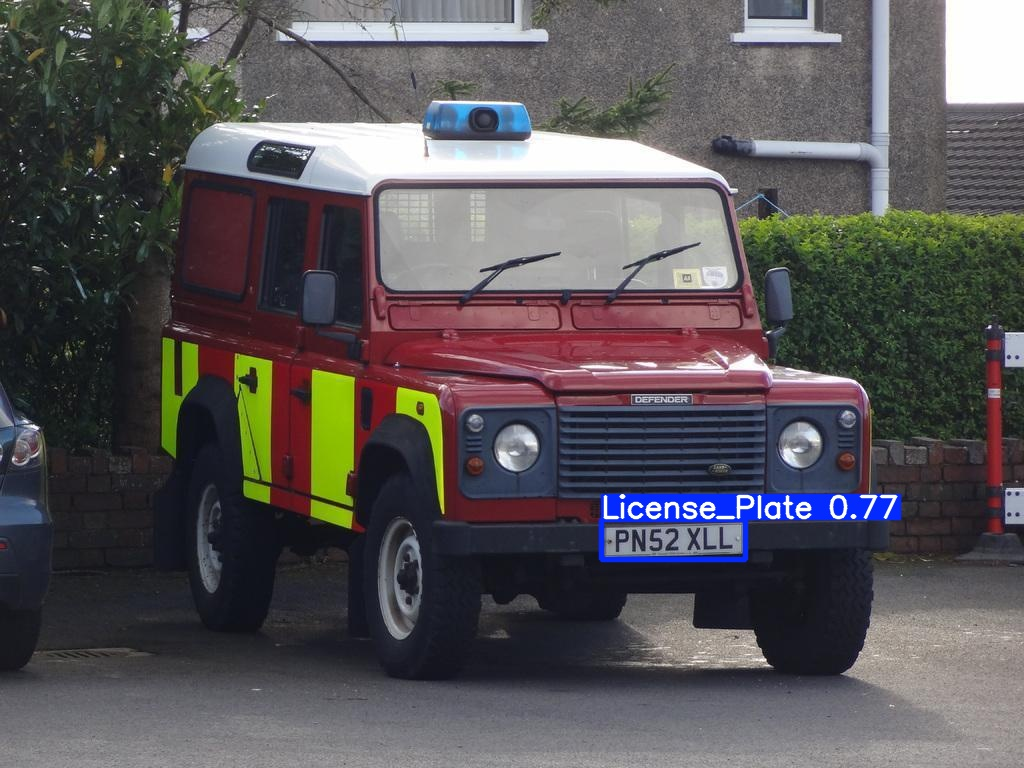
\includegraphics[width=\textwidth]{pics/TODO-car-wo-label.jpeg}

\vspace{0.2cm}

\end{columns}

\begin{center}
\begin{tikzpicture}[
    every node/.style={font=\scriptsize},
    num/.style={font=\ttfamily\large},
    def/.style={align=center, font=\scriptsize},
    arrow/.style={-Latex, thin}
]

% Numbers in the example label
\node[num] (class) at (0,0) {0};
\node[num] (xc)    at (1.2,0) {0.512};
\node[num] (yc)    at (2.8,0) {0.781};
\node[num] (w)     at (4.4,0) {0.154};
\node[num] (h)     at (6.0,0) {0.067};

% Definitions alternating above and below
\node[def, above=0.5cm of class] (classdef) {klasa obiektu};
\node[def, below=0.5cm of xc]    (xcdef)    {\texttt{x\_center}\\środek w poziomie};
\node[def, above=0.5cm of yc]    (ycdef)    {\texttt{y\_center}\\środek w pionie};
\node[def, below=0.5cm of w]     (wdef)     {\texttt{width}\\szerokość ramki};
\node[def, above=0.5cm of h]     (hdef)     {\texttt{height}\\wysokość ramki};

% Vertical arrows
\draw[arrow] (classdef) -- (class);
\draw[arrow] (xc) -- (xcdef);
\draw[arrow] (ycdef) -- (yc);
\draw[arrow] (w) -- (wdef);
\draw[arrow] (hdef) -- (h);

\end{tikzpicture}
\end{center}


\scriptsize
Wartości \texttt{x\_center}, \texttt{y\_center}, \texttt{width} i \texttt{height}
są znormalizowane do rozmiaru obrazu, czyli mają wartości od 0 do 1.

\end{frame}


%---------------------------------------------------------

\begin{frame}{Crop tablicy z marginesem}

Po wykryciu tablicy przez model YOLO wycinany jest fragment obrazu odpowiadający przewidzianej ramce ograniczającej.

\begin{itemize}
    \item Crop ogranicza dalsze przetwarzanie tylko do obszaru tablicy.
    \item Surowe cropy YOLO są bardzo ciasne -- znaki dotykają krawędzi, co pogarsza
    rozpoznawanie. Dlatego wycinamy tablice ponownie \textbf{z marginesem $\approx$12\%}
    wokół boxa.
    \item Każdy crop jest dodatkowo \textbf{wyrównywany pod kątem} obliczonym
    z linii znaków (deskew na etapie odczytu).
    \item Odrzucono wcześniejszą rektyfikację konturową (perspektywiczną) -- psuła
    dobre cropy i nie prostowała krzywych tablic.
\end{itemize}

\end{frame}

%---------------------------------------------------------

\begin{frame}{Etap 2 -- detekcja znaków (Char-YOLO)}

Drugi model wykrywa i klasyfikuje pojedyncze znaki na wyciętej tablicy.

\begin{itemize}
    \item Wariant \texttt{YOLO11s} (small, $\sim$9{,}4~mln parametrów) -- znaki są małe,
    większa sieć pomaga.
    \item 36 klas: cyfry \texttt{0--9} oraz litery \texttt{A--Z}.
    \item Większa rozdzielczość wejścia (\texttt{imgsz} = 480) zwiększa znaki na mapach cech.
    \item Po detekcji następuje \textbf{filtrowanie} (NMS + reguły geometryczne)
    i \textbf{sortowanie} znaków w naturalnej kolejności czytania.
    \item Obsługa tablic \textbf{dwurzędowych}: górny wiersz $\rightarrow$ dolny wiersz.
\end{itemize}

\vspace{0.2cm}

\footnotesize
\textbf{Problem:} dataset prawdziwych znaków jest mały (ok.\ 146 obrazów),
więc 36-klasowa detekcja uczona tylko na nich działa słabo. Rozwiązanie na kolejnych slajdach.

\end{frame}


\begin{frame}{\textit{License Plate Characters - Detection OCR} (F.~Pettini)}


Zawiera $\sim$200 tablic rejestracyjnych a na nich $\sim$2000 oznaczonych znaków.

Wykorzystany jako podstawa do ucznia odczytywania znaków oraz jako wyłączny zbiór walidacyjny i testowy.

\vspace{0.4cm}

\begin{figure}
    \centering
    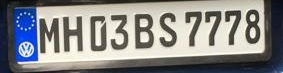
\includegraphics[width=0.4\textwidth]{pics/dataset2.png}

    \vspace{0.1cm}
    {\scriptsize Przykładowa tablica rejestracyjna z datasetu}
\end{figure}


\textbf{Etykiety znaków:} klasy \texttt{0--35} odpowiadające cyfrom \texttt{0--9}
oraz literom \texttt{A--Z} (\texttt{CHAR\_CLASSES}).


\end{frame}

%---------------------------------------------------------

\begin{frame}{Generator syntetycznych tablic}

Aby zwiększyć liczbę danych treningowych \textbf{bez ręcznego oznaczania},
zbudowano generator syntetycznych tablic.

\begin{itemize}
    \item Tablica renderowana jest \textbf{znak po znaku}, więc generator zna dokładne
    współrzędne każdego znaku $\rightarrow$ bounding boxy powstają automatycznie.
    \item Kolejność operacji:
    \begin{enumerate}
        \item render czystej tablicy + boxy znaków,
        
        \item transformacje \textbf{geometryczne} (perspektywa, rotacja) -- boxy
        przekształcane tą samą macierzą,
    
        \item degradacje \textbf{fotometryczne} (blur, szum, niska rozdzielczość, JPEG)
        -- nie zmieniające geometrii.
    \end{enumerate}
\end{itemize}

\begin{figure}
    \centering
    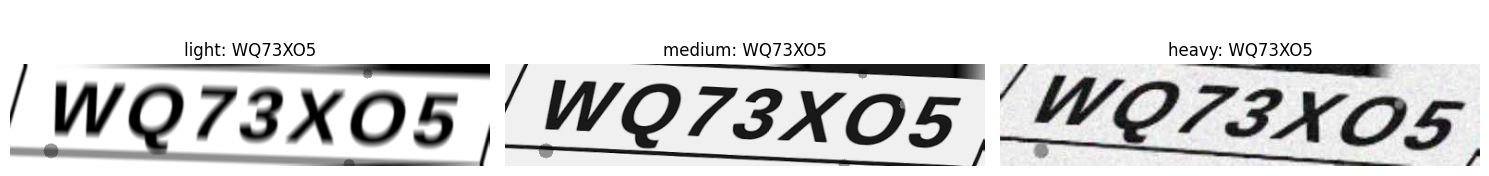
\includegraphics[width=\textwidth]{pics/syntatyki.png}
    \vspace{0.1cm}
    {\scriptsize Wizualizacja poziomów degradacji wygenerowanych tablic rejestracyjnych}
\end{figure}

\end{frame}



\begin{frame}{Generator syntetycznych tablic}

    Wygenerowano 12 000 obrazów (+ etykiety YOLO),
    w tym $\sim$30\% tablic dwurzędowych.

    \begin{figure}
        \centering
        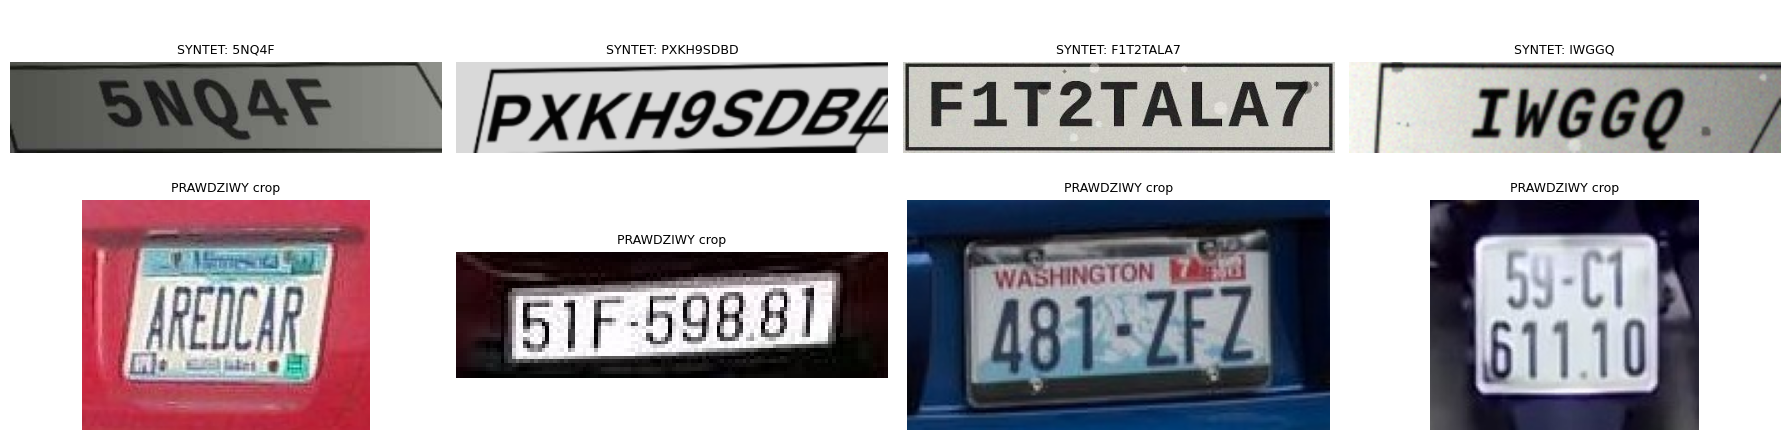
\includegraphics[width=0.8\textwidth]{pics/syntatyki2.png}

        {\scriptsize Porównanie syntetyków z prawdziwymi cropami}
    \end{figure}

    \begin{figure}
        \centering
        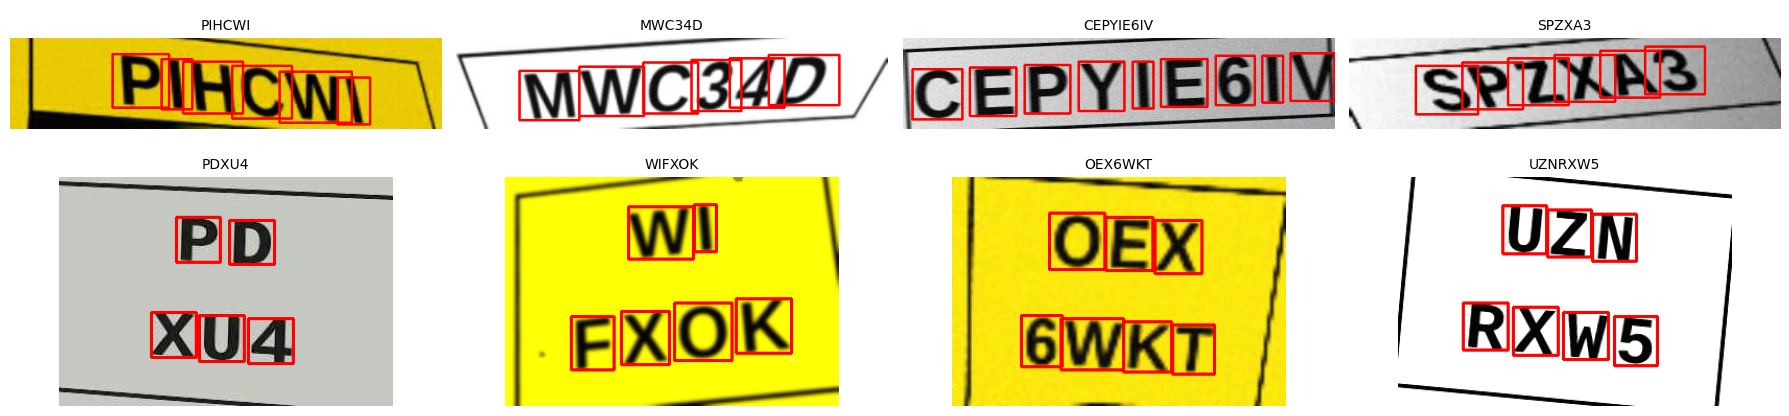
\includegraphics[width=0.8\textwidth]{pics/syntatyki3.png}

        {\scriptsize Syntetyki z zaznaczonymi bounding boxami cyfr}
    \end{figure}

    \footnotesize Syntetyki trafiają tylko do zbioru treningowego -- val/test pozostają
    w 100\% prawdziwe.

\end{frame}

%---------------------------------------------------------

\begin{frame}{Pseudo-etykietowanie (self-training)}

Trzecie źródło danych treningowych -- \textbf{za darmo}.

\begin{itemize}
    \item Trzeci dataset ma tysiące cropów z etykietami \textbf{tekstowymi},
    ale bez boxów znaków.
    \item \textbf{Trik:} przepuszczamy te cropy przez świeżo wytrenowany Char-YOLO.
    Jeśli odczytany ciąg \textbf{dokładnie zgadza się} z etykietą tekstową,
    to detekcje były poprawne $\rightarrow$ przewidziane boxy stają się nowymi
    etykietami treningowymi.
    \item Zgodność tekstu działa jak \textbf{automatyczny filtr jakości}
    (zła detekcja = zły tekst = odrzut). Próg pewności: \texttt{conf} = 0{,}50.
    \item Następnie dotrenowanie modelu o pseudo-etykiety
    
    (a więc syntetyki + 146 prawdziwych + pseudo-etykietowane).
\end{itemize}

\end{frame}

%---------------------------------------------------------

\begin{frame}{\textit{License Plate Text Recognition Dataset}
(N.~Yazdani)}

\begin{columns}[T,onlytextwidth]

% LEWA KOLUMNA
\column{0.6\textwidth}

Zawiera tysiące cropów tablic z etykietami \textbf{tekstowymi} (bez bounding boxów znaków).

\vspace{0.4cm}

\textbf{Etykiety znaków:} klasy \texttt{0--35} odpowiadające cyfrom \texttt{0--9}
oraz literom \texttt{A--Z} (\texttt{CHAR\_CLASSES}).

% KOLUMNA
\column{0.4\textwidth}
\begin{figure}
    \centering
    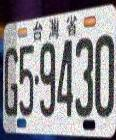
\includegraphics[width=0.7\textwidth]{pics/dataset3.jpg}

    \vspace{0.5cm}
    \texttt{\huge G59430}

    \vspace{0.1cm}
    {\scriptsize Przykładowa tablica rejestracyjna i jej etykieta}
\end{figure}

\end{columns}

\end{frame}


%---------------------------------------------------------
\section{Opis wdrożenia metod / modelu}
%---------------------------------------------------------

\begin{frame}{Opis wdrożenia metod / modelu}

\textbf{Środowisko chmurowe.} Notatnik wykrywa automatycznie środowisko
(Kaggle / Colab / lokalne) i ustawia ścieżki danych oraz zapisu wyników.
Trening prowadzono na GPU \textbf{Tesla T4} (Ultralytics 8.4, PyTorch + CUDA).

\vspace{0.3cm}

\textbf{Organizacja pipeline'u:}
\begin{itemize}
    \item Etap 1 (tablica) i Etap 2 (znaki) trenowane niezależnie; wagi zapisywane
    jako \texttt{plate\_detector\_best.pt} oraz \texttt{char\_yolo\_best.pt}.
    \item Możliwość pominięcia treningu przez wczytanie gotowych wag z wejścia
    (oszczędność czasu GPU).
    \item Oba modele pakowane do jednego ZIP-a do ponownego użycia / obrony.
\end{itemize}

\vspace{0.3cm}

\textbf{Postprocessing odczytu:} zamiana na wielkie litery, usunięcie spacji
i znaków specjalnych, pozostawienie wyłącznie \texttt{[A-Z0-9]}.
\\[2pt]
\footnotesize\texttt{"PCZ DSq8"} $\rightarrow$ \texttt{"PCZDSQ8"}

\end{frame}




%---------------------------------------------------------
\section{Wyniki}
%---------------------------------------------------------

\begin{frame}{Wyniki -- detekcja tablicy (YOLO11n)}

Metryki detekcji tablicy (jedna klasa \texttt{License\_Plate}):

\vspace{0.4cm}

\begin{center}
\begin{tabular}{lcccc}
\toprule
\textbf{Zbiór} & \textbf{Precision} & \textbf{Recall} & \textbf{mAP@0.5} & \textbf{mAP@0.5:0.95} \\
\midrule
Walidacyjny & 0{,}983 & 0{,}948 & 0{,}970 & 0{,}686 \\
Testowy     & 0{,}990 & 0{,}949 & 0{,}972 & 0{,}692 \\
\bottomrule
\end{tabular}
\end{center}

\vspace{0.4cm}

\begin{itemize}
    \item Bardzo wysoka skuteczność wykrywania samej tablicy (mAP@0.5 $\approx$ 0{,}97).
    \item Niższe mAP@0.5:0.95 wynika z surowszego progu IoU -- lokalizacja jest
    nieco mniej precyzyjna, ale w zupełności wystarcza do crop\-owania.
\end{itemize}

\end{frame}

%---------------------------------------------------------

\begin{frame}{Wyniki -- detekcja znaków (Char-YOLO)}

Metryki detekcji 36 klas znaków (val/test w 100\% prawdziwe):

\vspace{0.4cm}

\begin{center}
\begin{tabular}{lcccc}
\toprule
\textbf{Zbiór} & \textbf{Precision} & \textbf{Recall} & \textbf{mAP@0.5} & \textbf{mAP@0.5:0.95} \\
\midrule
Walidacyjny & 0{,}818 & 0{,}792 & 0{,}838 & 0{,}605 \\
Testowy     & 0{,}933 & 0{,}889 & 0{,}959 & 0{,}680 \\
\bottomrule
\end{tabular}
\end{center}

\vspace{0.4cm}

\begin{itemize}
    \item Dane syntetyczne + pseudo-etykietowanie pozwoliły wytrenować 36-klasowy
    detektor mimo małej liczby prawdziwych oznaczeń.
    \item Najtrudniejsze są znaki łatwe do pomylenia: \texttt{O}/\texttt{0},
    \texttt{Q}, \texttt{X}, \texttt{8}/\texttt{B}.
\end{itemize}

\end{frame}

%---------------------------------------------------------

\begin{frame}{Wyniki -- odczyt całej tablicy (tekst)}

Ewaluacja \textbf{tekstowa} na ręcznie oznaczonej próbce (\textbf{177 przykładów}):

\vspace{0.2cm}

\begin{center}
\begin{tabular}{lc}
\toprule
\textbf{Metryka} & \textbf{Wartość} \\
\midrule
Exact match (cała tablica poprawna) & 0{,}610 \\
Similarity (podobieństwo ciągów)    & 0{,}877 \\
CER (Character Error Rate)          & 0{,}147 \\
\bottomrule
\end{tabular}
\end{center}

\vspace{0.2cm}

\begin{itemize}
    \item Ok.\ \textbf{61\%} tablic odczytanych \textbf{w pełni poprawnie}.
    \item Średnio \textbf{$\sim$15\% znaków} z błędem (CER) -- najczęściej
    pojedyncza pomyłka na tablicę.
    \item Wysokie \emph{similarity} (0{,}88) oznacza, że nawet błędne odczyty
    są zwykle bliskie prawdziwemu numerowi.
\end{itemize}

\vspace{0.2cm}

\footnotesize
\textit{CER = odległość edycyjna / długość ground truth (im niżej, tym lepiej).}

\end{frame}





%---------------------------------------------------------
\section{Wnioski}
%---------------------------------------------------------


\begin{frame}{Wnioski}

\begin{itemize}
    \item Dwustopniowy pipeline oparty na \texttt{YOLO11} \textbf{skutecznie odczytuje
    tablice} -- detekcja tablicy niemal bezbłędna (mAP@0.5 $\approx$ 0{,}97).
    \item \textbf{Dane syntetyczne} okazały się kluczowe: pozwoliły obejść problem
    małego zbioru oznaczonych znaków bez ręcznego etykietowania.
    \item \textbf{Pseudo-etykietowanie} dostarczyło dodatkowych, darmowych prawdziwych
    danych, a zgodność tekstu zadziałała jak automatyczny filtr jakości.
    \item Wąskim gardłem pozostaje \textbf{etap odczytu znaków} (61\% exact match):
    pojedyncze pomyłki na trudnych/krzywych tablicach obniżają dokładność całej tablicy.
\end{itemize}

\vspace{0.3cm}

\textbf{Kierunki dalszych prac:}
\begin{itemize}
    \footnotesize
    \item więcej i bardziej realistycznych syntetyków (czcionki, tła, degradacje),
    \item lepsza rektyfikacja silnie przekrzywionych tablic,
    \item walidacja formatu numeru (reguły rejestracji) jako postprocessing.
\end{itemize}

\end{frame}


\begin{frame}
\centering
\vfill
{\Large Dziękujemy za uwagę}
\vfill
\end{frame}


\end{document}
